\documentclass[12pt,a4paper]{article}
\usepackage[utf8]{inputenc}
\usepackage{polski}
\usepackage[polish]{babel}
\usepackage{graphicx}
\usepackage{hyperref}
\usepackage[margin=2.5cm]{geometry}
\usepackage{listings}
\usepackage{xcolor}
\usepackage{amsmath}
\usepackage{enumitem}
\usepackage{tikz}
\usepackage{float}
\usepackage{svg}
\usepackage{titlesec}


\titleclass{\subsubsubsection}{straight}[\subsubsection]
\newcounter{subsubsubsection}[subsubsection]
\renewcommand\thesubsubsubsection{\thesubsubsection.\arabic{subsubsubsection}}
\titleformat{\subsubsubsection}
  {\normalfont\normalsize\bfseries}{\thesubsubsubsection}{1em}{}
\titlespacing*{\subsubsubsection}{0pt}{3.25ex plus 1ex minus .2ex}{1.5ex plus .2ex}

\setcounter{tocdepth}{4}

\definecolor{codegreen}{rgb}{0,0.6,0}
\definecolor{codegray}{rgb}{0.5,0.5,0.5}
\definecolor{codepurple}{rgb}{0.58,0,0.82}
\definecolor{backcolour}{rgb}{0.95,0.95,0.95}

\lstdefinestyle{mystyle}{
	backgroundcolor=\color{backcolour},   
	commentstyle=\color{codegreen},
	keywordstyle=\color{blue},
	stringstyle=\color{codepurple},
	basicstyle=\ttfamily\scriptsize,
	breakatwhitespace=false,         
	breaklines=true,                 
	captionpos=b,                    
	keepspaces=true,                 
	numbersep=5pt,                  
	showspaces=false,                
	showstringspaces=false,
	showtabs=false,                  
	tabsize=2
}

\lstset{style=mystyle}

\begin{document}

\begin{titlepage}
\begin{center}
\large
    {\noindent Collegium Witelona Uczelnia Państwowa w Legnicy}\\
    {\noindent Wydział Nauk Technicznych i Ekonomicznych}\\
    {\noindent Kierunek: Informatyka}\\[2cm]
    
\includegraphics[width=5cm]{godlo.jpg}\\[2cm]
    {\large\textbf{Projekt z przedmiotu "Projektowanie i programowanie systemów internetowych I"}}\\[0.3cm]
    {\noindent Temat: Faily.}\\[3cm]
    {\large\textbf{Autorzy}}\\
    Mateusz Bogacz-Drewniak, nr. indeksu: 44491\\
    Gabriela Grabarska, nr. indeksu: 43840\\
    Mateusz Chimkowski, nr. indeksu: 43831\\[2.5cm]			
\end{center}
		
\begin{flushright}
    \begin{tabular}{l}
        Prowadzący przedmiot\\
        mgr inż. Krzysztof Rewak
    \end{tabular}
\end{flushright}
		
\vfill
\begin{center}
    {\noindent Legnica, 2025}
    \end{center}
\end{titlepage}

\tableofcontents
\newpage

\section{Cel i ogólna charakterystyka projektu}

Projekt Faily to webowa aplikacja przygotowana jako zaliczenie przedmiotu „Projektowanie i programowanie systemów internetowych" na drugim roku studiów.

\subsection{Główne cele projektu}

Celem projektu jest umożliwienie użytkownikom:
\begin{itemize}[itemsep=0pt]
    \item zawierania nowych znajomości,
    \item organizowania spotkań z poznanymi już osobami,
    \item zarządzania wydarzeniami i ofertami wspólnych eventów,
    \item organizowania wspólnych dojazdów do miejsc z konkretnymi wydarzeniami.
\end{itemize}

\newpage

\begin{figure}[H]
    \centering
    \resizebox{15cm}{22cm}{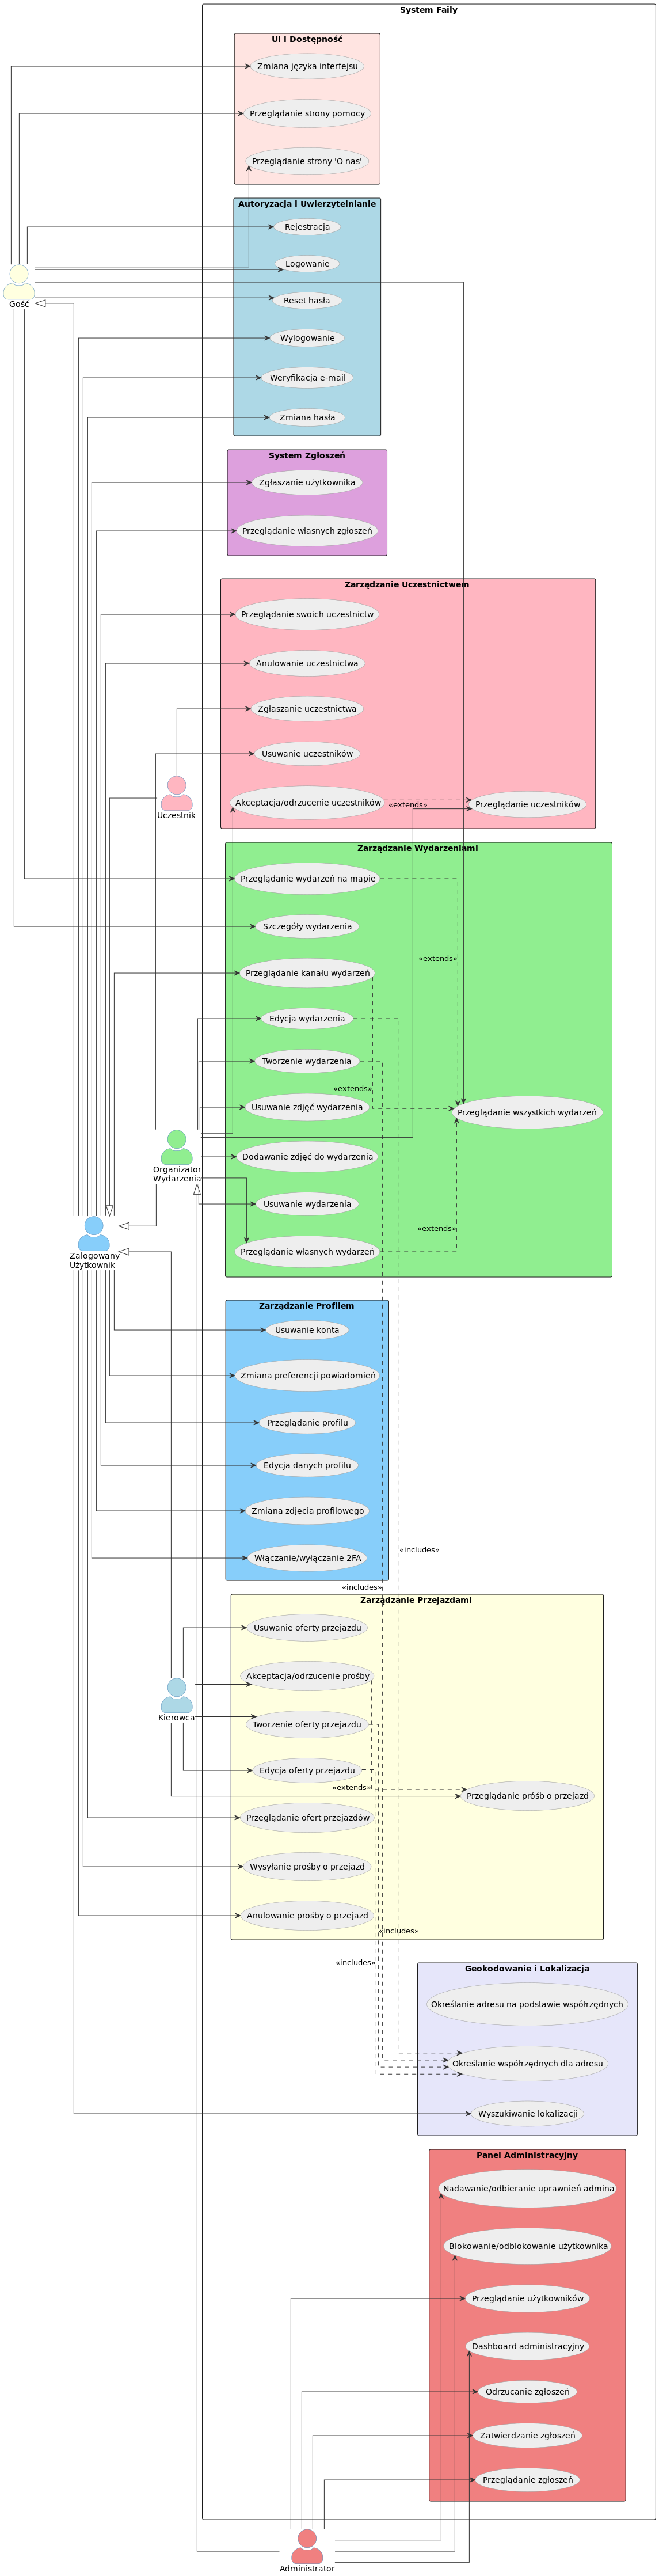
\includegraphics{use_case_diagram.png}}
    \caption{Diagram przypadków użycia(opracowanie własne)}
    \label{fig:diagram-klas}
\end{figure}

\newpake

\subsection{Funkcjonalność systemu}

System pozwala użytkownikom na:
\begin{itemize}[itemsep=0pt]
    \item rejestrację w systemie,
    \item tworzenie wydarzeń,
    \item przeglądanie wydarzeń (na mapie, w panelu aktualności lub stronie postów),
    \item zgłaszanie udziału w wydarzeniach,
    \item tworzenie i wysyłanie próśb o wspólny dojazd na wydarzenia.
\end{itemize}

\section{Wnioski projektowe}

W trakcie realizacji projektu napotkano szereg wyzwań, które dostarczyły cennych doświadczeń dla przyszłych projektów.

\subsection{Główne wyzwania}

\begin{enumerate}[itemsep=3pt]
    \item \textbf{Aspekty programistyczne} -- Napotkano znaczące wyzwania związane z implementacją złożonych funkcjonalności systemu.
    
    \item \textbf{Komunikacja zespołowa} -- Komunikacja w zespole wymagała usprawnienia, szczególnie w zakresie koordynacji zadań.
    
    \item \textbf{Harmonogram projektu} -- Pierwotny harmonogram stwarzał nadmierne obciążenie dla członków zespołu.
    
    \item \textbf{Podział kompetencji} -- Podział zadań nie był optymalny względem kompetencji członków zespołu.
    
    \item \textbf{Złożoność projektu} -- Faktyczna złożoność projektu przewyższyła wstępne szacunki dotyczące wymaganych zasobów.
    
    \item \textbf{Kompatybilność technologii} -- Wybór frameworka frontend niezgodnego z domyślnym stosem Laravel spowodował znaczne trudności w integracji z gotowymi komponentami autoryzacji (Laravel Breeze), wymagając dodatkowych nakładów na dostosowanie interfejsu.
\end{enumerate}

\subsection{Możliwości ulepszenia działania}

Na podstawie zdobytych doświadczeń, w przyszłości warto:
\begin{enumerate}[itemsep=3pt]
    \item Wybierać technologie frontend kompatybilne z frameworkiem backend, aby uniknąć problemów integracyjnych i skrócić czas developmentu.
    \item Lepiej podzielić role w zespole ze względu na wiedzę i doświadczenie członków.
    \item Dokładniej oszacować złożoność projektu na etapie planowania.
    \item Wdrożyć lepsze praktyki komunikacji zespołowej.
\end{enumerate}

\section{Struktura katalogów i plików projektu}

Projekt został zorganizowany zgodnie z konwencjami Laravel, co ułatwia nawigację po kodzie i rozszerzanie funkcjonalności.

\subsection{Główne pliki konfiguracyjne}

\begin{itemize}[itemsep=2pt]
    \item \textbf{compose.yaml} -- główny plik Docker Compose opisujący usługi aplikacji (kontener aplikacji, bazy danych, Redis, Mailpit).
    \item \textbf{environment/dev/app/} -- pliki konfiguracyjne dla kontenera aplikacji: Dockerfile, konfiguracje Nginx, PHP-FPM, Supervisor.
\end{itemize}

\subsection{Struktura kodu aplikacji}

\subsubsection{Katalog src/}
Główny katalog kodu aplikacji Laravel zawiera:

\textbf{src/app/} -- kod aplikacji obejmujący:
\begin{itemize}[itemsep=1pt]
    \item \textbf{Http/Controllers/} -- kontrolery odpowiadające za logikę HTTP (kontroler eventów, uwierzytelniania, API, geokodowania)
    \item \textbf{Models/} -- modele Eloquent (User, Event, EventAttendee, Ride, Photo)
    \item \textbf{Repositories/} -- klasy dostępu do danych (EventRepository, UserRepository)
    \item \textbf{Services/} -- warstwa serwisowa pośrednicząca między kontrolerami a repozytoriami
    \item \textbf{Notifications/} -- klasy powiadomień (wysyłanie e-maili przypomnień)
\end{itemize}

\subsubsection{Pozostałe katalogi}

\begin{itemize}[itemsep=2pt]
    \item \textbf{src/config/} -- pliki konfiguracyjne Laravel (baza danych, cache, mail, autoryzacja)
    
    \item \textbf{src/database/} -- migracje, seedy i fabryki bazy danych
    
    \item \textbf{src/public/} -- publiczny katalog projektu (index.php, zasoby statyczne)
    
    \item \textbf{src/resources/} -- zasoby frontendowe i widoki:
    \begin{itemize}[itemsep=1pt]
        \item \textbf{views/} -- szablony Blade (autoryzacja, panel użytkownika, formularze)
        \item \textbf{css/} -- główny plik CSS/SCSS importujący Bootstrap
        \item \textbf{js/} -- pliki JavaScript i Vue (komponenty, konfiguracja Vite)
    \end{itemize}
    
    \item \textbf{src/routes/} -- definicje tras (web.php dla tras webowych)
    
    \item \textbf{src/storage/} -- pliki cache, logi i uploady użytkowników
    
    \item \textbf{src/tests/} -- testy jednostkowe i funkcjonalne
\end{itemize}

\newpage

\begin{figure}[H]
    \centering
    \resizebox{15cm}{20cm}{\rotatebox{90}{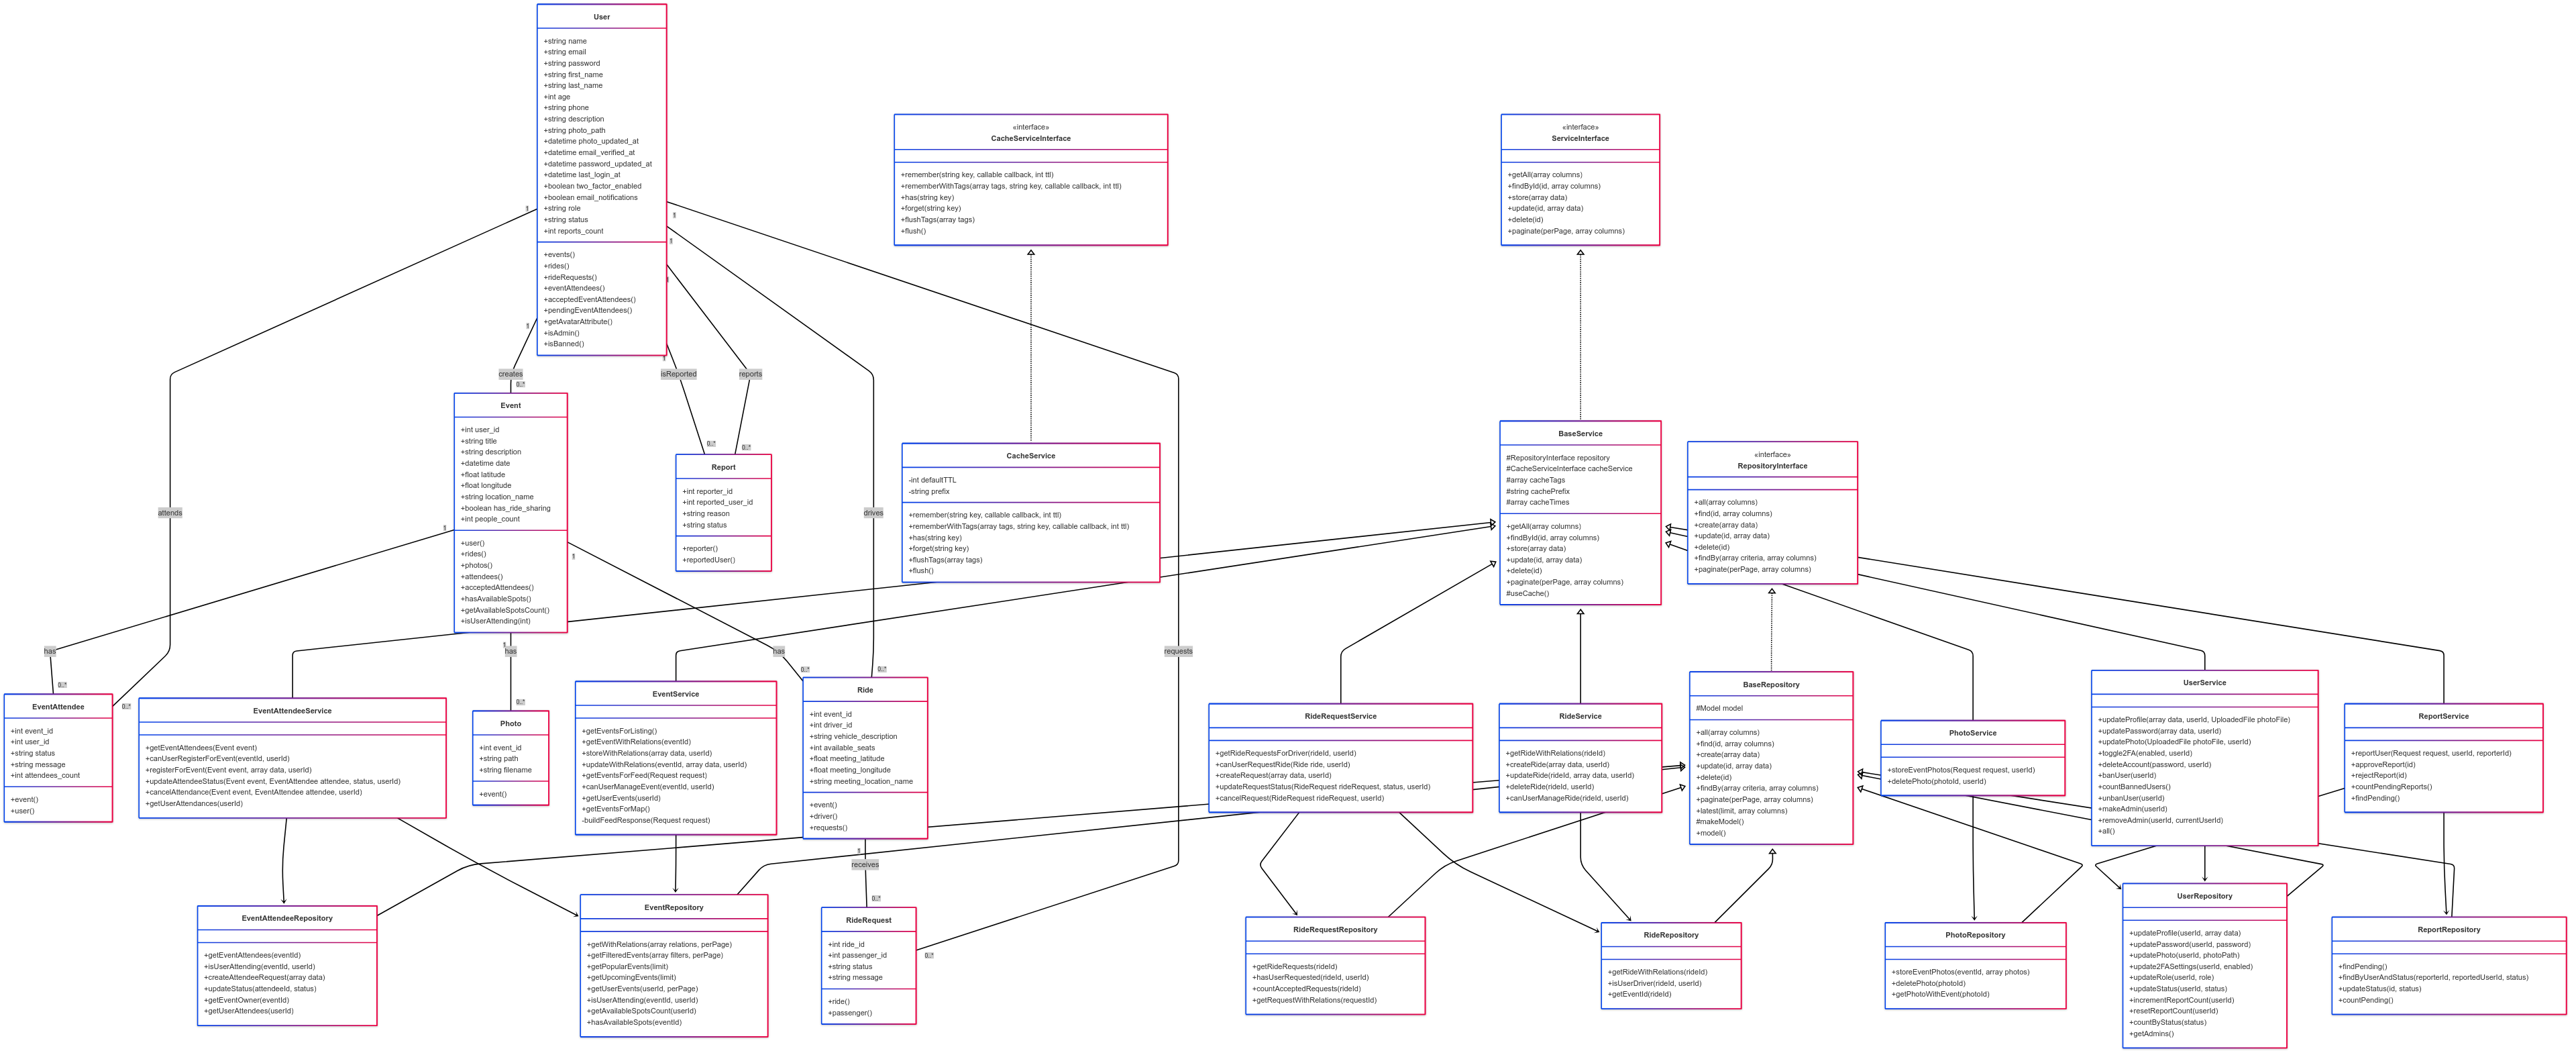
\includegraphics{class_diagram.png}}}
    \caption{Diagram klas systemu (opracowanie własne)}
    \label{fig:diagram-klas}
\end{figure}

\newpage

\section{Użyte technologie i frameworki}

Dokładne zestawienie wykorzystanych technologii przedstawia poniższa tabela:

\begin{table}[H]
\centering
\begin{tabular}{@{}p{4cm}p{8cm}@{}}
\toprule
\textbf{Technologia} & \textbf{Opis wykorzystania} \\
\midrule
Laravel (backend) & Struktura MVC, Eloquent ORM \\
PHP & Wersja 8.3 w kontenerze Docker \\
Composer & Menedżer pakietów PHP \\
NPM & Node.js 18 + Vite 6.x do budowania frontendu \\
Bootstrap & Framework CSS do responsywnego UI \\
Vue.js & Interaktywne komponenty frontend (Vite, plugin Vue) \\
vue-i18n & Obsługa wielojęzyczności po stronie Vue \\
Leaflet & Wyświetlanie i interakcja z mapami \\
PostgreSQL & Relacyjna baza danych (kontener postgres:17-alpine) \\
Redis & Cache, sesje (kontener redis:7.4-alpine) \\
Laravel Sanctum & Uwierzytelnianie i autoryzacja API \\
Predis & Klient PHP do współpracy z Redis \\
Mailpit & Lokalny serwer SMTP do testów e-maili \\
Spatie ActivityLog & Logowanie aktywności użytkowników i modeli \\
Axios & Biblioteka HTTP do asynchronicznych wywołań API \\
Laravel Breeze & System autoryzacji (Blade + Bootstrap) \\
Docker Compose & Konfigurowanie środowiska wielokontenerowego \\
\bottomrule
\end{tabular}
\caption{Wykorzystane technologie i frameworki}
\end{table}

Powyższe technologie zostały dobrane w celu kompleksowej realizacji funkcji webowej aplikacji. Laravel zapewnia solidne API i logikę serwera, Bootstrap i Vue odpowiadają za interaktywny, responsywny interfejs. Docker gwarantuje spójną konfigurację środowiska deweloperskiego.

\newpage

\section{Opis działania poszczególnych komponentów}

\subsection{Kontrolery (Controllers)}

W katalogu \texttt{src/app/Http/Controllers/} znajdują się klasy obsługujące żądania HTTP:

\subsubsection{Upsttrolery}
\begin{itemize}
    \item \textbf{EventController} -- operacje CRUD dla wydarzeń, tworzenie i edycja wydarzeń z obsługą współdzielenia przejazdów, wyświetlanie feedu wydarzeń z filtrowaniem i paginacją
    \item \textbf{EventAttendeeController} -- zarządzanie uczestnictwem w wydarzeniach, rejestracja uczestników, akceptacja/odrzucanie zgłoszeń, wyświetlanie listy uczestników dla organizatorów
    \item \textbf{UserAttendancesController} -- wyświetlanie listy wydarzeń, w których użytkownik bierze udział
    \item \textbf{RideController} -- operacje CRUD dla przejazdów, tworzenie ofert przejazdu dla wydarzeń z określeniem miejsca spotkania i liczby dostępnych miejsc
    \item \textbf{RideRequestController} -- zarządzanie zgłoszeniami do przejazdów, składanie wniosków o przejazd, akceptacja/odrzucanie przez kierowców
    \item \textbf{ProfileController} -- zarządzanie profilem użytkownika, edycja danych osobowych, zmiana zdjęcia profilowego, aktywacja 2FA, usuwanie konta
    \item \textbf{UserSettingsController} -- ustawienia użytkownika, zmiana hasła, aktualizacja danych kontaktowych
    \item \textbf{BannedController} -- obsługa zbanowanych użytkowników, wyświetlanie informacji o banie
    \item \textbf{AdminController} -- panel administracyjny, zarządzanie użytkownikami (banowanie/odbanowywanie), nadawanie uprawnień administratora, przeglądanie statystyk
    \item \textbf{ReportController} -- system zgłoszeń, moderacja zgłoszeń użytkowników, zatwierdzanie/odrzucanie raportów o niepożądanych zachowaniach
    \item \textbf{GeocodingController} -- pobieranie adresów i lokalizacji za pomocą API Nominatim OpenStreetMap, wyszukiwanie miejsc i reverse geocoding
    \item \textbf{PhotoController} -- zarządzanie zdjęciami wydarzeń, dodawanie i usuwanie zdjęć przez organizatorów
    \item \textbf{MainMapController} -- wyświetlanie mapy z wydarzeniami, pobieranie danych o lokalizacjach wydarzeń
    \item \textbf{LanguageController} -- zarządzanie językami interfejsu, przełączanie między dostępnymi lokalizacjami (pl, en, jpn, es, ua)
\end{itemize}

\subsubsection{Kontrolery API}
W katalogu \texttt{Api/} znajduje się zestaw kontrolerów udostępniających REST API pod prefiksem \texttt{/api}. Każdy kontroler obsługuje operacje CRUD oraz dodatkowe endpointy, zabezpieczone middlewarem \texttt{auth:sanctum}.

\subsection{Kontlolery Auth}
W katalogu \texttt{auth/} znajduje się zestaw kontrolerów dostarczonych przez Laravel Breeze, które umożliwiają kompletną obsługę uwierzytelniania użytkowników -- rejestrację, logowanie, weryfikację email, resetowanie haseł oraz potwierdzanie tożsamości dla operacji wymagających dodatkowego bezpieczeństwa.

\subsection{Modele (Models)}

W katalogu \texttt{src/app/Models/} znajdują się klasy Eloquent odpowiadające tabelom bazy danych:

\begin{itemize}[itemsep=2pt]
    \item \textbf{User} -- model użytkownika z funkcją powiadomień
    \item \textbf{Event} -- model wydarzenia
    \item \textbf{EventAttendee} -- model uczestnictwa w wydarzeniu
    \item \textbf{Ride} -- model oferty dojazdu
    \item \textbf{RideRequest} -- model prośby o dojazd
    \item \textbf{Photo} -- model zdjęć
    \item \textbf{Report} -- model zgłoszeń użytkowników
\end{itemize}

Modele zawierają relacje i metody pomocnicze, wykorzystując Eloquent ORM do łatwego wykonywania operacji na bazie danych.

\subsection{System tras (Routing)}

\subsubsection{Trasy webowe (web.php)}
Generują widoki HTML, obejmują:
\begin{itemize}[itemsep=1pt]
    \item logowanie i rejestrację,
    \item listę i widok pojedynczego wydarzenia,
    \item panel użytkownika,
    \item strony statyczne („O nas", „Pomoc").
\end{itemize}

\subsubsection{Trasy API (api.php)}
REST API z prefiksem \texttt{/api}, zawierające publiczne punkty końcowe do rejestracji i logowania. Pozostałe trasy zabezpieczone middlewarem \texttt{auth:sanctum}.

\subsection{Widoki i szablony (Blade Templates)}

W katalogu \texttt{resources/views/} znajdują się pliki Blade:

\begin{itemize}[itemsep=2pt]
    \item \textbf{Autoryzacja} -- formularze logowania, rejestracji, resetu hasła
    \item \textbf{Wydarzenia} -- lista, tworzenie, edycja wydarzeń
    \item \textbf{Komponenty pomocnicze} -- navbar, footer
    \item \textbf{Strony dodatkowe} -- centrum pomocy, widok mapy
\end{itemize}

\subsection{Komponenty Vue.js}

W katalogu \texttt{resources/js/components/} znajdują się komponenty:

\begin{itemize}[itemsep=2pt]
    \item \textbf{LeafletMap.vue} -- interaktywna mapa do przeglądania wydarzeń z markerami, wyszukiwaniem miejsc, geolokalizacją i popup'ami ze szczegółami eventów
    \item \textbf{EventForm.vue} -- kompleksowy formularz tworzenia wydarzeń z dwoma mapami (lokalizacja wydarzenia i miejsce spotkania dla car sharing), wyszukiwaniem adresów, upload'em zdjęć i geokodowaniem
\end{itemize}

\subsection{Cache i kolejki}

System wykorzystuje Redis jako domyślny store dla cache'u, sesji i kolejek. Powiadomienia e-mail są kolejkowane, a worker'y Supervisor obsługują kolejkę w tle.

\subsection{System logowania}

Oprócz standardowego logowania Laravel, projekt wykorzystuje pakiet Spatie Activitylog, który zapisuje aktywność użytkowników do osobnej tabeli. Umożliwia to śledzenie zdarzeń w systemie (np. tworzenie/usuwanie obiektów).

\subsection{System mailingu}

Konfiguracja SMTP wysyła e-maile do serwera Mailpit, który udostępnia interfejs webowy do podglądu wiadomości. Wykorzystano mechanizm powiadomień Laravel (np. EventReminderNotification).

\newpage

\begin{figure}[H]
    \centering
    \resizebox{15cm}{20cm}{\rotatebox{90}{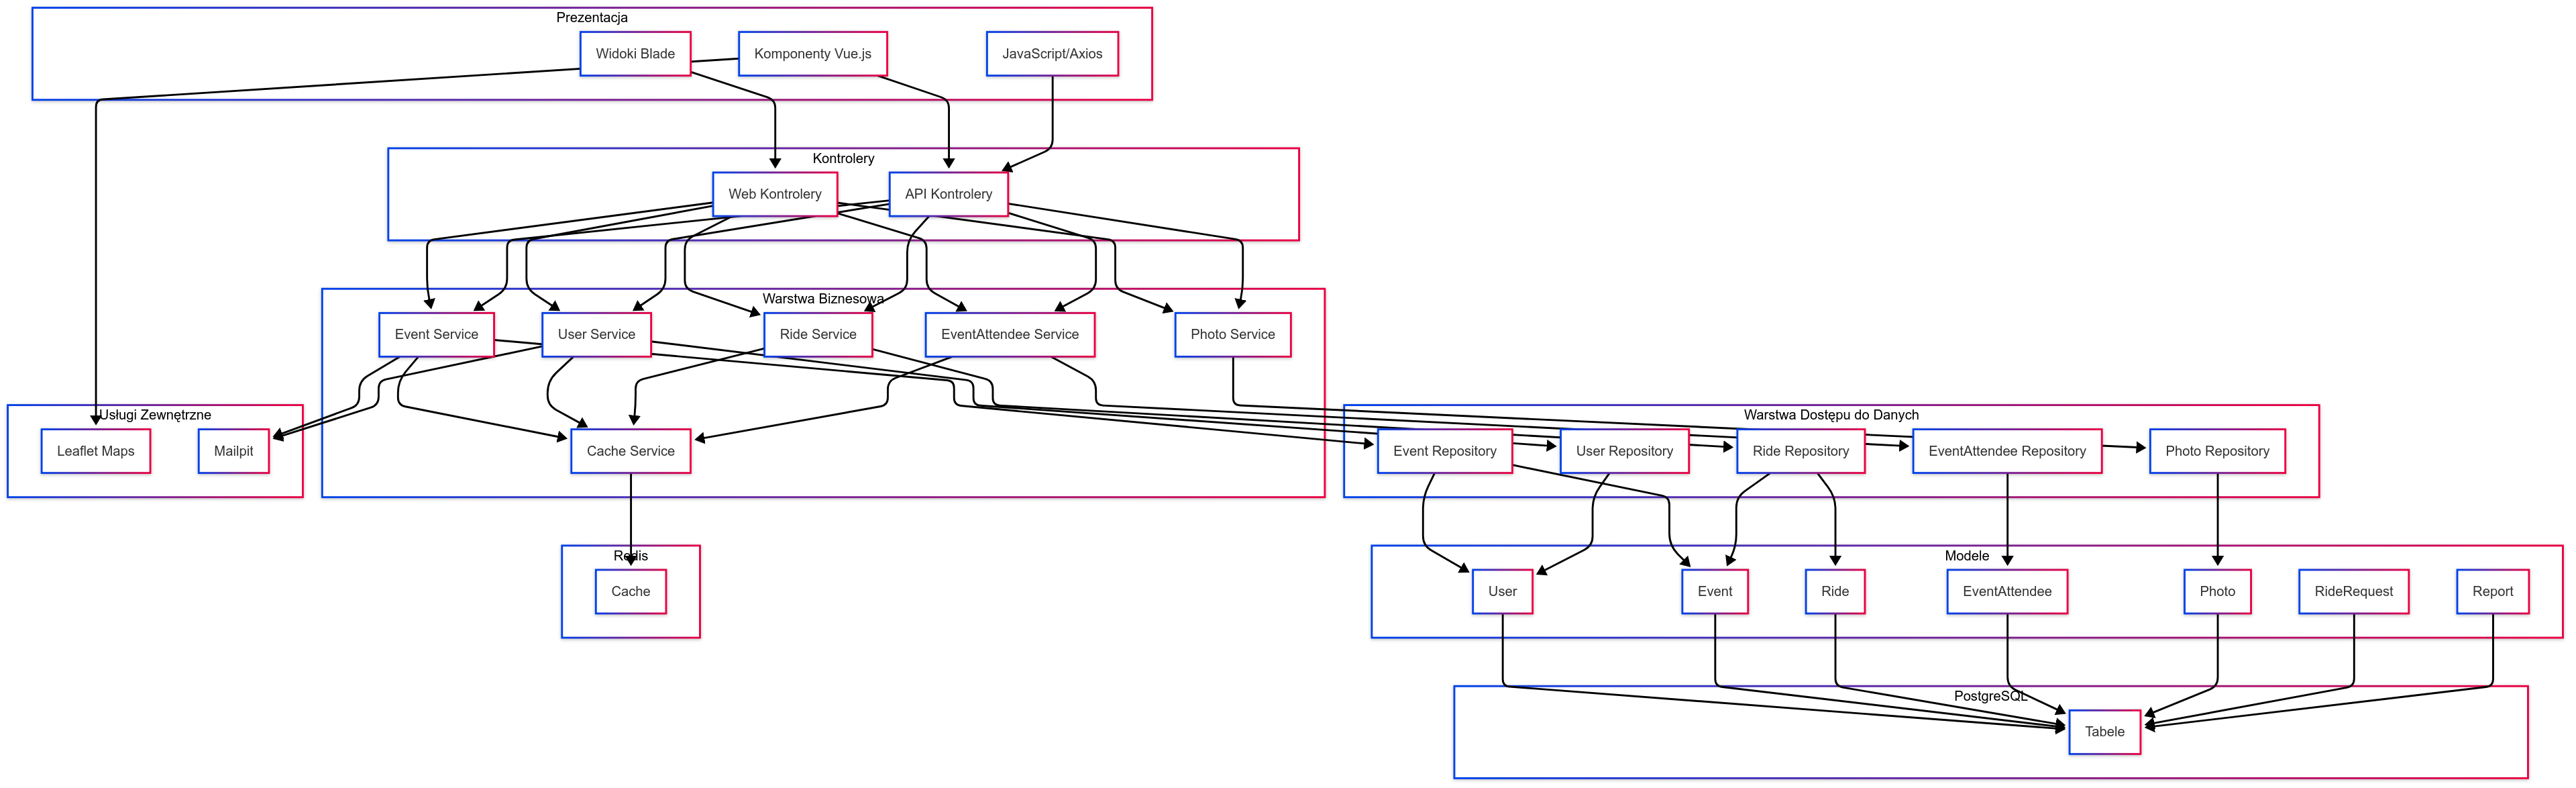
\includegraphics{component_diagram.png}}}
    \caption{Diagram komponentów (opracowanie własne)}
    \label{fig:diagram-klas}
\end{figure}

\newpage

\section{Konfiguracja Docker, bazy danych i zależności}

Projekt wykorzystuje Docker Compose z następującymi usługami:

\subsection{Usługa app}
Główny kontener z aplikacją Laravel, zbudowany na bazie obrazu PHP. Instalowane są dodatkowe rozszerzenia PHP (gd, pgsql, zip, redis, xdebug), Nginx i Supervisor. Port 80 mapowany na hosta (domyślnie 63851).

\subsection{Usługa database}
Kontener PostgreSQL 17 z trwałymi danymi dzięki wolumenowi \texttt{faily-postgres-data}. Port 5432 mapowany na hosta (domyślnie 63853).

\subsection{Usługa redis}
Kontener Redis używany jako cache i do przechowywania sesji Laravel. Dane trwałe dzięki wolumenowi \texttt{faily-redis-data}. Port 6379 mapowany na hosta (domyślnie 63852).

\subsection{Usługa mailpit}
Testowy serwer SMTP z interfejsem webowym na porcie 8025 (domyślnie host 63854). Aplikacja Laravel wysyła e-maile na port SMTP Mailpit (1025).

Plik \texttt{compose.yaml} definiuje wszystkie usługi oraz sieć \texttt{faily-dev}. Kontener aplikacji zależy od bazy danych i sprawdza jej stan przed startem.

\newpage

\begin{figure}[H]
    \centering
    \resizebox{15cm}{20cm}{
        \rotatebox{90}
        {
            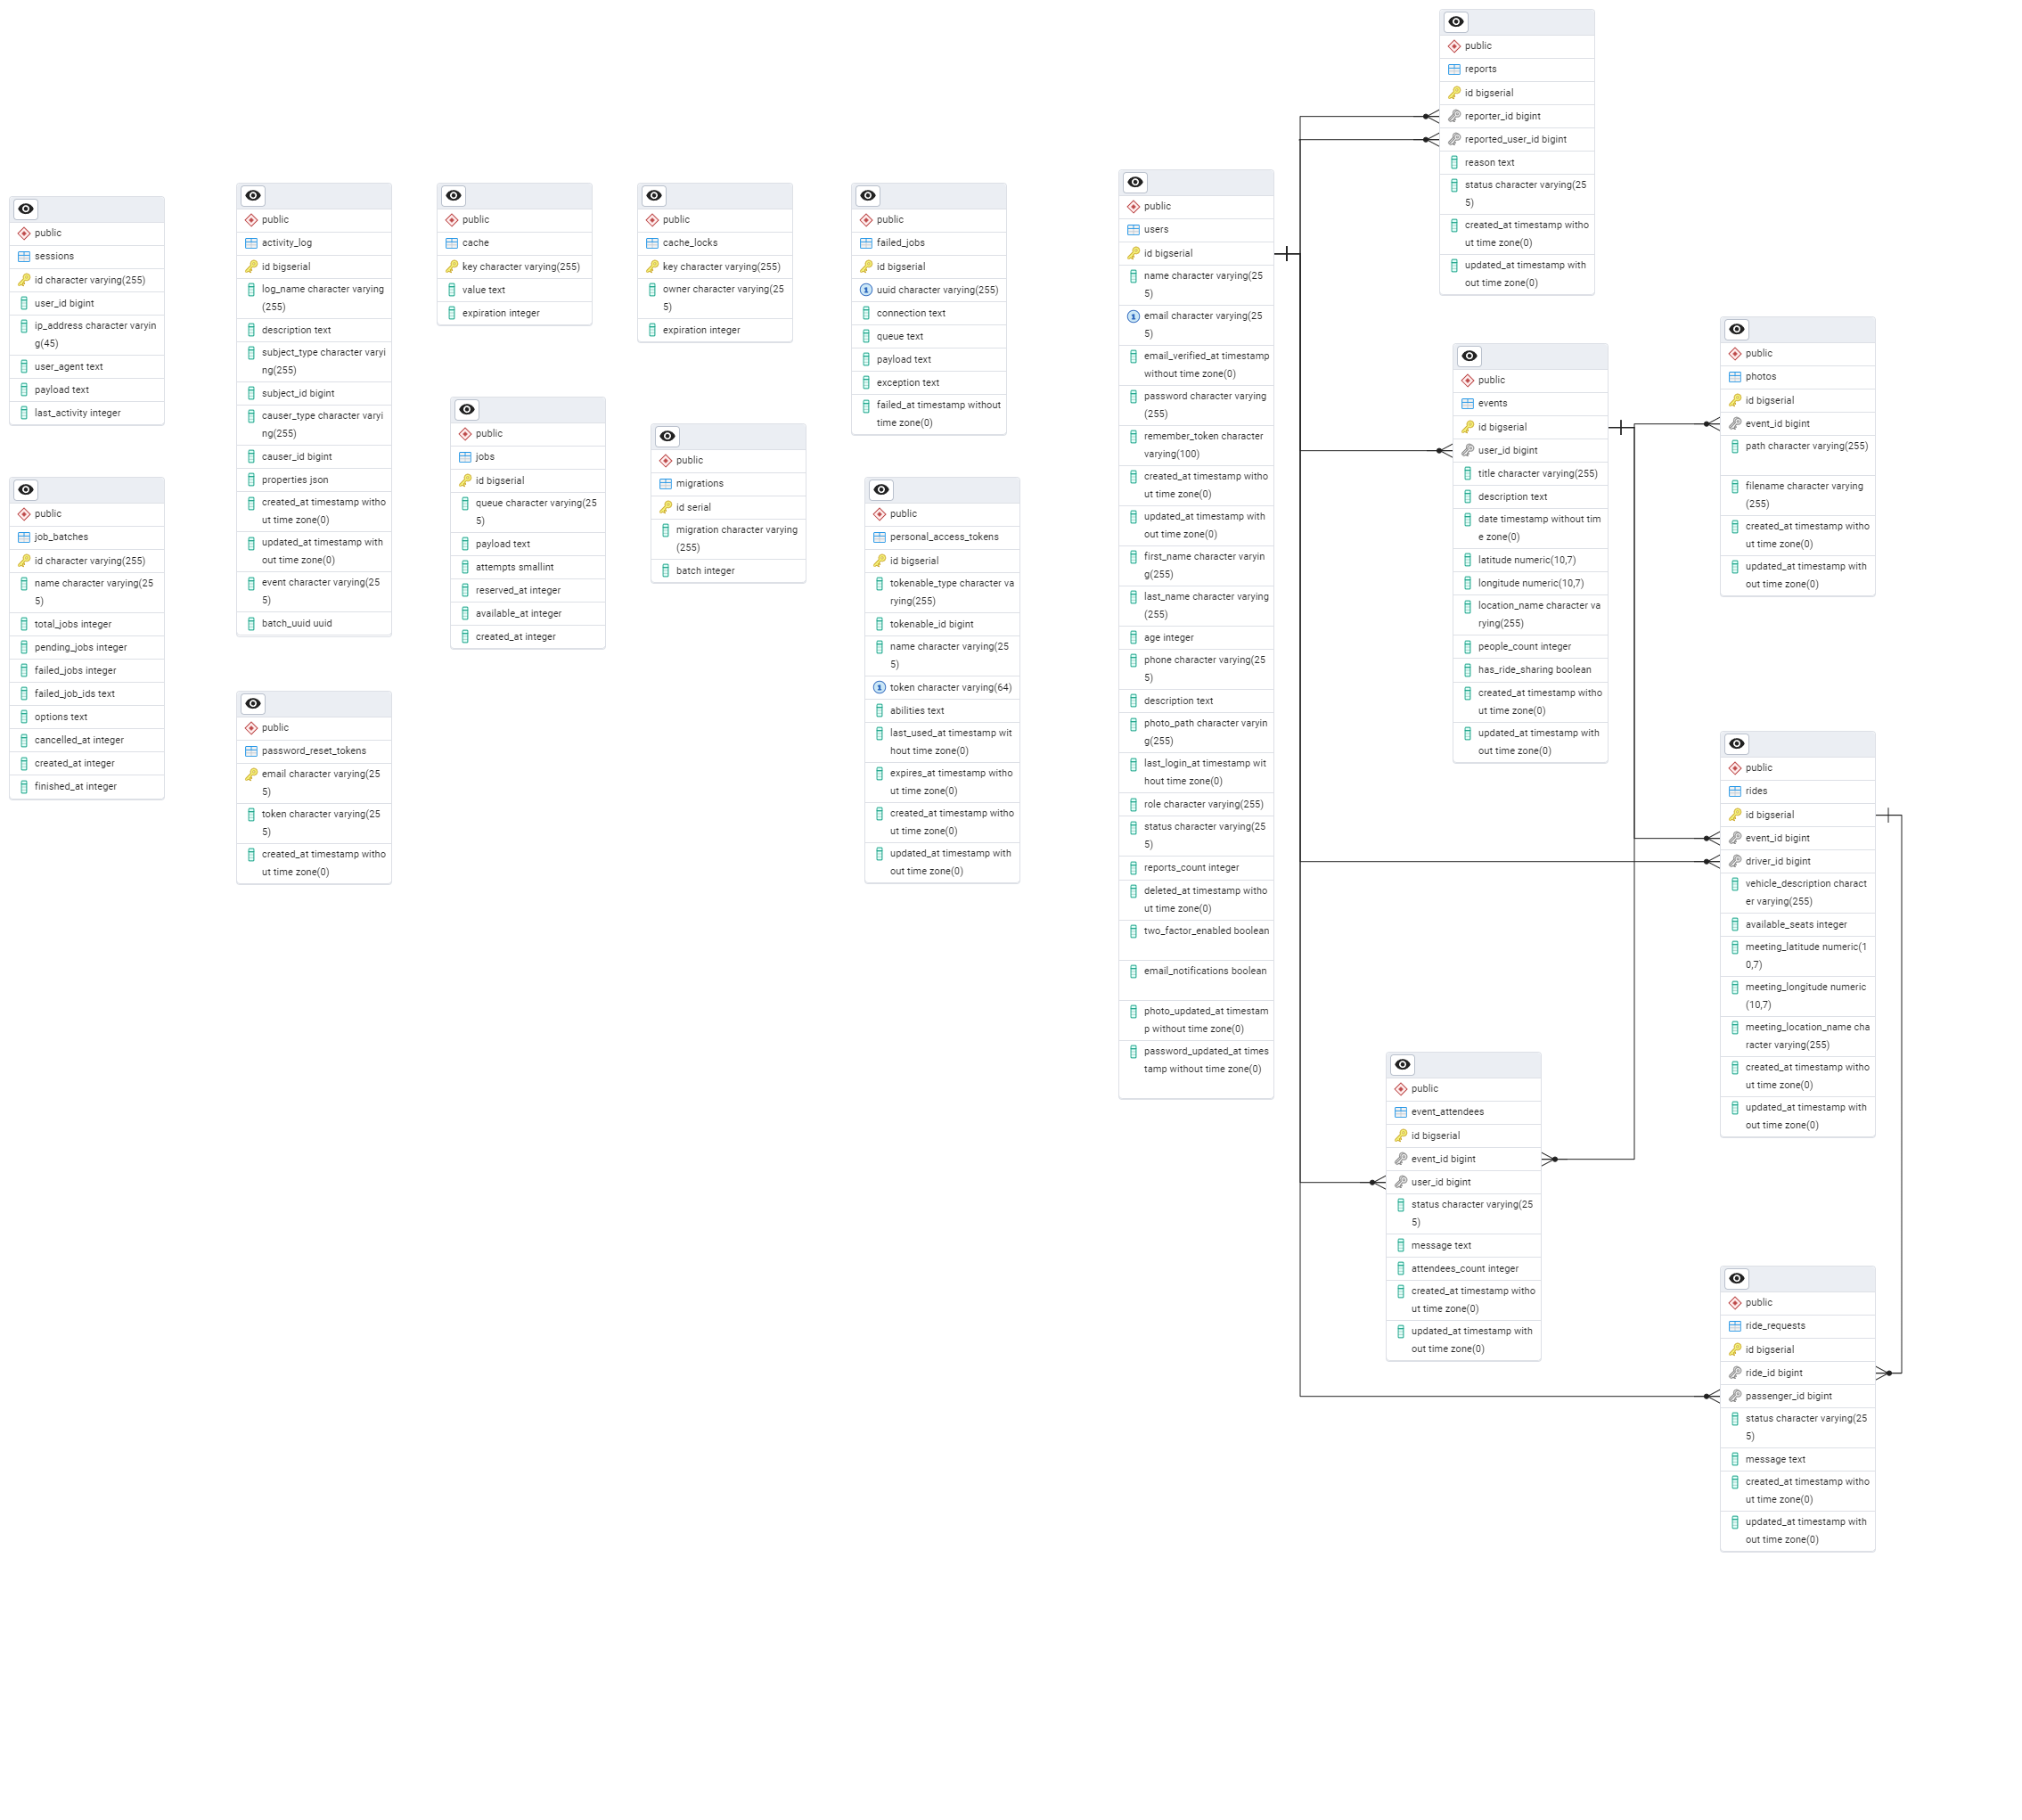
\includegraphics{Faily_ERD.png}
        }
    }
    \caption{Diagram ERD projektu Faily (opracowanie własne)}
    \label{fig:diagram-erd}
\end{figure}

\newpage

\section{Analiza wdrożonych systemów}

\subsection{Założenia projektowe}

Projekt realizuje następujące założenia techniczne:

\begin{enumerate}[itemsep=3pt]
    \item \textbf{Framework MVC} -- Aplikacja wykorzystuje Laravel 12 implementujący wzorzec Model-View-Controller.
    
    \item \textbf{Framework CSS} -- Bootstrap 5 zapewnia responsywny i spójny wygląd interfejsu.
    
    \item \textbf{Baza danych} -- PostgreSQL 17 jako relacyjna baza danych z dostępem przez Eloquent ORM.
    
    \item \textbf{Cache} -- Redis jako pamięć podręczna, sesje i kolejki.
    
    \item \textbf{Dependency Manager} -- Composer dla backendu (PHP), NPM dla frontendu (JavaScript).
    
    \item \textbf{HTML} -- Blade do generowania widoków HTML z wbudowanymi zmiennymi Laravel.
    
    \item \textbf{CSS} -- Bootstrap 5 uzupełniony własnymi stylami w \texttt{app.css}.
    
    \item \textbf{JavaScript} -- Vue.js jako główny framework z komponentami i Axios do komunikacji API.
    
    \item \textbf{Routing} -- Laravel dla tras serwera (web.php)
    
    \item \textbf{ORM} -- Eloquent ORM mapujący tabele na modele PHP z relacjami.
    
    \item \textbf{Uwierzytelnianie} -- Laravel Breeze + Laravel Sanctum dla API.
    
    \item \textbf{lokalizacja} -- System tłumaczeń Laravel z folderami \texttt{resources/lang/} oraz wykożustanie i18n dla tłumaczeń elementów Vue.
    
    \item \textbf{Mailing} -- Powiadomienia Laravel z integracją Mailpit do testów.
    
    \item \textbf{Formularze} -- Formularze HTML Blade z tokenami CSRF i walidacją.
    
    \item \textbf{Interakcje Asynchroniczne} -- Vue.js + Axios do operacji bez przeładowania strony.
    
    \item \textbf{Konsumowanie API} -- Integracja z Nominatim OSM do geokodowania.
    
    \item \textbf{Publikacja API} -- REST API pod prefiksem \texttt{/api} z kontrolerami CRUD.
    
    \item \textbf{RWD} -- Bootstrap + meta viewport dla wszystkich urządzeń.
    
    \item \textbf{Logger} -- Laravel logs + Spatie Activitylog do audytu.
    
    \item \textbf{Deployment} -- Wdrożenie zostało zrealizowane z wykorzystaniem Docker Compose, z przygotowanymi skryptami oraz szczegółową instrukcją zawartą w dokumentacji. Aplikacja została wdrożona w środowisku produkcyjnym w chmurze Oracle Cloud, z użyciem Laravel, Vue, Nginx oraz innych niezbędnych komponentów. Dodatkowo, w ramach wdrożenia wykorzystano: darmową wersję Upstash dla usługi Redis, darmową wersję Supabase opartą na PostgreSQL oraz bezpłatną wersję Brevo do obsługi wysyłki wiadomości e-mail.

\end{enumerate}

\section{Przebieg działania aplikacji}

\subsection{Przykładowe scenariusze użytkownika}

\subsubsection{Rejestracja i logowanie}
Użytkownik wypełnia formularz rejestracji, Laravel tworzy nowego użytkownika i wysyła e-mail potwierdzający. Po potwierdzeniu można się zalogować -- sesja jest utrzymywana po stronie serwera, a token Sanctum przyznawany przy logowaniu mobilnym.

\subsubsection{Przeglądanie wydarzeń}
Na stronie /event_list użytkownik widzi listę nadchodzących wydarzeń w postaci kart Bootstrap. Może filtrować wydarzenia i przejść do szczegółów.

\subsubsection{Tworzenie wydarzeń}
Zalogowany użytkownik przechodzi do formularza tworzenia wydarzeń. Dzięki komponentowi mapy może wpisać adres i otrzymać sugestię lokalizacji (geokodowanie). Po zapisaniu dane trafiają do bazy, a autor może edytować wydarzenie.

\subsubsection{Uczestnictwo w wydarzeniu}
Na stronie wydarzenia znajduje się przycisk zgłoszenia udziału. Po wciśnięciu tworzony jest wpis w bazie. Organizator może zaakceptować lub odrzucić zgłoszenie przez interfejs aplikacji.

\subsubsection{Prośby o wspólny dojazd}
Użytkownik może przeglądać oferty przejazdów lub utworzyć własną. W widoku wydarzenia znajduje się sekcja „Dojazd" z formularzem. Po wpisaniu punktów początkowego i docelowego użytkownik wysyła prośbę. Właściciel może zaakceptować lub odrzucić prośbę.

\subsubsection{Panel administracyjny}
Przygotowano folder \texttt{resources/views/admin/} z plikami panelu administratora do zarządzania użytkownikami i eventami.

\subsubsection{Zmiana języka}
W navbarze znajduje się przełącznik języka. Po wyborze interfejs przeładowuje się z odpowiednimi tłumaczeniami, a Vue przełącza język komponentów.

\newpage

\section{Uruchomienie aplikacji lokalnielokalne}

\subsection{Wymagania wstępne}

Do uruchomienia aplikacji wymagane są:
\begin{itemize}[itemsep=1pt]
    \item Docker
    \item Docker Compose
    \item Git
\end{itemize}

\subsection{Proces instalacji}

\subsubsection{Klonowanie repozytorium}
\begin{lstlisting}[language=bash, caption=Pobranie kodu źródłowego]
git clone https://github.com/mateusz-bogacz-collegiumwitelona/Faily/
cd Faily
\end{lstlisting}

\subsubsection{Przygotowanie środowiska}

Upewnij się, że porty \texttt{63851}, \texttt{63852}, \texttt{63853}, \texttt{63854} oraz \texttt{5173} są dostępne. Następnie zmień nazwy plików \texttt{.env.example} na \texttt{.env} w katalogu głównym projektu oraz w katalogu \textbf{src}. Po wykonaniu tych czynności można przystąpić do budowania obrazu Dockera:

\begin{lstlisting}[language=bash, caption=Uruchomienie kontenerów]
docker-compose build
docker-compose up
\end{lstlisting}

\subsubsection{Konfiguracja projektu}

\textbf{Opcja automatyczna (skrypt)}:
\begin{lstlisting}[language=bash, caption=Użycie skryptu konfiguracyjnego]
docker exec -it faily-app-dev bash
chmod +x deploy.sh
./deploy.sh
\end{lstlisting}

\textbf{Opcja manualna}:
\begin{lstlisting}[language=bash, caption=Konfiguracja manualna]
docker exec -it faily-app-dev bash
composer install
npm install
npm run build
php artisan migrate
php artisan key:generate
php artisan db:seed
php artisan storage:link
\end{lstlisting}

\subsection{Dostęp do aplikacji}

Po zakończeniu instalacji aplikacja będzie dostępna pod adresami:
\begin{itemize}[itemsep=1pt]
    \item \textbf{Aplikacja Laravel}: \url{http://localhost:63851}
    \item \textbf{Panel Mailpit}: \url{http://localhost:63854}
\end{itemize}

\newpage

\section{Wdrożenie aplikacji na serwerze}

\subsection{Wprowadzenie}

Instrukcja opisuje proces wdrożenia aplikacji Laravel+Vue.js na serwerze VPS z Ubuntu, wykorzystujący zewnętrzne usługi:
\begin{itemize}[itemsep=1pt]
    \item \textbf{Supabase} -- baza danych PostgreSQL
    \item \textbf{Upstash} -- cache Redis
    \item \textbf{Brevo} -- wysyłanie e-maili
\end{itemize}

\subsection{Wymagania}

\begin{itemize}[itemsep=1pt]
    \item Serwer VPS z Ubuntu 24.04 (w projekcie: Oracle Cloud -- 1 rdzeń, 2 wątki, 16GB RAM, 50GB dysk)
    \item Dostęp SSH do serwera
    \item Skonfigurowane domeny (w projekcie: faily.pl i faily.online z home.pl)
    \item Konta w zewnętrznych usługach: Supabase, Upstash, Brevo
\end{itemize}

\subsection{Przygotowanie środowiska serwerowego}

\subsubsection{Aktualizacja systemu}
\begin{lstlisting}[language=bash, caption=Aktualizacja Ubuntu i instalacja pakietów]
sudo apt update && sudo apt upgrade -y
sudo apt install -y curl git unzip nginx supervisor certbot python3-certbot-nginx
\end{lstlisting}

\subsubsection{Instalacja PHP 8.3}
\begin{lstlisting}[language=bash, caption=Instalacja PHP i rozszerzeń]
sudo apt install -y software-properties-common
sudo add-apt-repository ppa:ondrej/php -y
sudo apt update

sudo apt install -y php8.3-fpm php8.3-cli php8.3-common \
php8.3-pgsql php8.3-mbstring php8.3-xml php8.3-zip \
php8.3-bcmath php8.3-gd php8.3-curl php8.3-redis
\end{lstlisting}

\subsubsection{Instalacja Node.js}
\begin{lstlisting}[language=bash, caption=Instalacja Node.js 18.x]
curl -fsSL https://deb.nodesource.com/setup_18.x | sudo -E bash -
sudo apt install -y nodejs
\end{lstlisting}

\subsubsection{Instalacja Composer}
\begin{lstlisting}[language=bash, caption=Instalacja Composer]
curl -sS https://getcomposer.org/installer | sudo php -- \
    --install-dir=/usr/local/bin --filename=composer
\end{lstlisting}

\subsubsection{Pobieranie kodu i ustawienie uprawnień}
\begin{lstlisting}[language=bash, caption=Przygotowanie katalogów i uprawnień]
sudo mkdir /var/www/faily 
cd /var/www/faily
git clone https://github.com/mateusz-bogacz-collegiumwitelona/Faily/ .

sudo mkdir -p storage/framework/{views,cache,sessions}

sudo chown ubuntu:www-data /var/www/faily
sudo chown -R www-data:www-data storage bootstrap/cache

sudo chmod 755 /var/www/faily
sudo chmod -R 775 storage bootstrap/cache
\end{lstlisting}

\subsubsection{Konfiguracja Nginx}
\begin{lstlisting}[language=bash, caption=Utworzenie konfiguracji Nginx]
sudo nano /etc/nginx/sites-available/faily
\end{lstlisting}

Zawartość pliku konfiguracyjnego:
\begin{lstlisting}[caption=Konfiguracja Nginx z SSL]
server {
    listen 80;
    server_name faily.pl www.faily.pl faily.online www.faily.online;
    return 301 https://$host$request_uri;
}

server {
    listen 443 ssl;
    server_name faily.pl www.faily.pl faily.online www.faily.online;

    ssl_certificate /etc/letsencrypt/live/faily.online/fullchain.pem;
    ssl_certificate_key /etc/letsencrypt/live/faily.online/privkey.pem;
    include /etc/letsencrypt/options-ssl-nginx.conf;
    ssl_dhparam /etc/letsencrypt/ssl-dhparams.pem;

    root /var/www/faily/src/public;
    index index.php index.html;

    location / {
        try_files $uri $uri/ /index.php?$query_string;
    }

    location ~ \.php$ {
        include snippets/fastcgi-php.conf;
        fastcgi_pass unix:/var/run/php/php8.3-fpm.sock;
        fastcgi_param SCRIPT_FILENAME $document_root$fastcgi_script_name;
        include fastcgi_params;
    }

    location ~ /\.(?!well-known).* {
        deny all;
    }
}
\end{lstlisting}

Aktywacja konfiguracji:
\begin{lstlisting}[language=bash, caption=Aktywacja konfiguracji Nginx]
sudo ln -s /etc/nginx/sites-available/faily /etc/nginx/sites-enabled/
sudo nginx -t
sudo systemctl restart nginx
\end{lstlisting}

\subsubsection{Konfiguracja PHP-FPM}

Utworzenie dedykowanego pool dla aplikacji:
\begin{lstlisting}[language=bash, caption=Konfiguracja PHP-FPM pool]
sudo nano /etc/php/8.3/fpm/pool.d/faily.conf
\end{lstlisting}

Zawartość pliku konfiguracyjnego:
\begin{lstlisting}[caption=Konfiguracja pool PHP-FPM]
[faily]
user = www-data
group = www-data
listen = /var/run/php/php8.3-fpm.sock
listen.owner = www-data
listen.group = www-data
pm = dynamic
pm.max_children = 10
pm.start_servers = 3
pm.min_spare_servers = 2
pm.max_spare_servers = 5
pm.process_idle_timeout = 10s
pm.max_requests = 500
\end{lstlisting}

Optymalizacja ustawień PHP:
\begin{lstlisting}[language=bash, caption=Optymalizacja PHP]
sudo nano /etc/php/8.3/fpm/conf.d/99-laravel.ini
\end{lstlisting}

\begin{lstlisting}[caption=Ustawienia optymalizacji]
upload_max_filesize = 100M
post_max_size = 100M
max_execution_time = 300
memory_limit = 512M
\end{lstlisting}

Restart usługi PHP:
\begin{lstlisting}[language=bash]
sudo systemctl restart php8.3-fpm
\end{lstlisting}

\subsubsection{Rekordy DNS}
W panelu zarządzania domeną należy dodać następujące rekordy:

\begin{table}[H]
\centering
\begin{tabular}{@{}lll@{}}
\toprule
\textbf{Typ} & \textbf{Nazwa} & \textbf{Wartość} \\
\midrule
A & @ & Adres IP serwera VPS \\
A & www & Adres IP serwera VPS \\
\bottomrule
\end{tabular}
\caption{Rekordy DNS do konfiguracji}
\end{table}

\newpage

\subsubsection{Certyfikat SSL}

Sprawdzenie propagacji DNS:
\begin{lstlisting}[language=bash, caption=Weryfikacja DNS]
dig faily.pl
dig www.faily.pl
dig faily.online  
dig www.faily.online
\end{lstlisting}

Uzyskanie certyfikatu SSL:
\begin{lstlisting}[language=bash, caption=Instalacja certyfikatu Let's Encrypt]
sudo systemctl stop nginx
sudo certbot certonly --standalone \
    -d faily.pl -d www.faily.pl \
    -d faily.online -d www.faily.online
sudo systemctl start nginx
\end{lstlisting}

\subsubsection{Instalacja zależności aplikacji}

\begin{lstlisting}[language=bash, caption=Instalacja zależności]
cd /var/www/faily/src
composer install --no-dev --optimize-autoloader
npm install
npm run build
\end{lstlisting}

\subsubsection{Przygotowanie pliku .env}
\begin{lstlisting}[language=bash, caption=Konfiguracja środowiska]
cp .env.example .env
php artisan key:generate
\end{lstlisting}

\newpage

\textbf{Przykładowa konfiguracja .env}
\begin{lstlisting}[caption=Plik .env dla produkcji]
APP_NAME=Faily
APP_ENV=production
APP_KEY=base64:wygenerowany_klucz
APP_DEBUG=false
APP_URL=https://faily.pl

APP_LOCALE=pl
APP_FALLBACK_LOCALE=en

# Konfiguracja bazy danych (Supabase)
DB_CONNECTION=pgsql
DB_HOST=host_podany_w_supabase
DB_PORT=port_podany_w_supabase
DB_DATABASE=nazwa_bazy_supabase
DB_USERNAME=uzytkownik_supabase
DB_PASSWORD=haslo_supabase

# Konfiguracja Redis (Upstash)
REDIS_CLIENT=predis
REDIS_HOST=host_podany_przez_upstash
REDIS_PASSWORD=haslo_podane_przez_upstash
REDIS_PORT=port_podany_przez_upstash
CACHE_DRIVER=redis
SESSION_DRIVER=redis
QUEUE_CONNECTION=redis

# Konfiguracja poczty (Brevo)
MAIL_MAILER=smtp
MAIL_HOST=host_podany_przez_brevo
MAIL_PORT=port_podany_przez_brevo
MAIL_USERNAME=nazwa_uzytkownika_brevo
MAIL_PASSWORD=haslo_brevo
MAIL_ENCRYPTION=tls
MAIL_FROM_ADDRESS=team@faily.pl
MAIL_FROM_NAME=Faily
\end{lstlisting}

\subsubsection{Konfiguracja Supervisor dla kolejek}

Utworzenie konfiguracji worker'a:
\begin{lstlisting}[language=bash, caption=Konfiguracja Supervisor]
sudo nano /etc/supervisor/conf.d/faily-worker.conf
\end{lstlisting}

\begin{lstlisting}[caption=Konfiguracja Laravel worker]
[program:faily-worker]
process_name=%(program_name)s_%(process_num)02d
command=php /var/www/faily/src/artisan queue:work --sleep=3 --tries=3
autostart=true
autorestart=true
user=www-data
numprocs=2
redirect_stderr=true
stdout_logfile=/var/log/faily-worker.log
stopwaitsecs=3600
\end{lstlisting}

Aktywacja Supervisor:
\begin{lstlisting}[language=bash, caption=Uruchomienie worker'a]
sudo supervisorctl reread
sudo supervisorctl update
sudo supervisorctl start faily-worker:*
\end{lstlisting}

\subsubsection{Optymalizacja aplikacji}
\begin{lstlisting}[language=bash, caption=Optymalizacja Laravel]
php artisan migrate --force
php artisan optimize
php artisan config:cache
php artisan route:cache
php artisan view:cache
php artisan storage:link
\end{lstlisting}

\subsubsection{Weryfikacja działania}
\begin{lstlisting}[language=bash, caption=Sprawdzenie statusu usług]
sudo systemctl status nginx php8.3-fpm
curl https://faily.pl
\end{lstlisting}

\subsection{Najczęstsze problemy i rozwiązania}

\begin{itemize}[itemsep=3pt]
    \item \subsubsection{Błędy uprawnień}Sprawdź uprawnienia katalogów \texttt{storage} i \texttt{bootstrap/cache}:
    \begin{lstlisting}[language=bash]
sudo chown -R www-data:www-data storage bootstrap/cache
sudo chmod -R 775 storage bootstrap/cache
    \end{lstlisting}
    
    \item \subsubsection{Błędy SSL} Upewnij się, że porty 80 i 443 są otwarte. Sprawdź ustawienia VNIC lub firewall:
    \begin{lstlisting}[language=bash]
sudo ufw allow 80
sudo ufw allow 443
    \end{lstlisting}
    
    \item \subsubsection{Błędy bazy danych} Zweryfikuj konfigurację Supabase w pliku \texttt{.env} oraz połączenie:
    \begin{lstlisting}[language=bash]
php artisan tinker
DB::connection()->getPdo();
    \end{lstlisting}
    
    \item \subsubsection{Błędy cache}Sprawdź konfigurację Upstash Redis:
    \begin{lstlisting}[language=bash]
php artisan cache:clear
php artisan config:clear
    \end{lstlisting}
    
    \item \subsubsection{Błędy e-mail} Zweryfikuj konfigurację Brevo i domenę nadawcy w pliku \texttt{.env}.
\end{itemize}

\subsection{Monitoring i logowanie}

Logi aplikacji znajdują się w:
\begin{itemize}[itemsep=1pt]
    \item \texttt{/var/www/faily/src/storage/logs/} -- logi Laravel
    \item \texttt{/var/log/nginx/} -- logi Nginx
    \item \texttt{/var/log/faily-worker.log} -- logi kolejek
\end{itemize}

\newpage

\section{Podsumowanie}

Projekt Faily stanowi kompleksową aplikację webową do zarządzania wydarzeniami, zrealizowaną z wykorzystaniem nowoczesnych technologii i najlepszych praktyk programistycznych.

\subsection{Osiągnięte cele}

Aplikacja pomyślnie realizuje wszystkie założone cele:
\begin{itemize}[itemsep=2pt]
    \item \textbf{Zarządzanie wydarzeniami} -- pełny cykl życia eventów
    \item \textbf{System użytkowników} -- rejestracja, autoryzacja, profile
    \item \textbf{Interakcje społeczne} -- uczestnictwo, wspólne dojazdy
    \item \textbf{Geolokalizacja} -- integracja z mapami i API geokodowania
    \item \textbf{Wielojęzyczność} -- obsługa multiple języków
    \item \textbf{Responsywność} -- działanie na różnych urządzeniach
\end{itemize}

\subsection{Wartości edukacyjne}

Projekt dostarczył zespołowi cennych doświadczeń w zakresie:
\begin{itemize}[itemsep=2pt]
    \item pracy z frameworkiem Laravel i ekosystemem PHP,
    \item integracji frontendu (Vue.js) z backendem,
    \item konfiguracji środowiska Docker,
    \item wdrażania aplikacji na serwerze produkcyjnym,
    \item pracy zespołowej nad złożonym projektem.
\end{itemize}

\subsection{Możliwości rozwoju}

Aplikacja stanowi solidną podstawę do dalszego rozwoju. Potencjalne usprawnienia obejmują:
\begin{itemize}[itemsep=2pt]
    \item implementację aplikacji mobilnej,
    \item rozszerzenie funkcji społecznościowych,
    \item integrację z zewnętrznymi serwisami społecznościowymi,
    \item zaawansowaną analitykę użytkowników,
    \item dodanie możliwości ocenianie wydarzeń i użytkowników,
\end{itemize}

Dzięki wykorzystaniu sprawdzonych technologii i architektury MVC, aplikacja jest przygotowana na skalowanie i dalszy rozwój funkcjonalności.

\newpage
\listoffigures

\newpage
\renewcommand{\lstlistlistingname}{Spis kodów źródłowych}
\lstlistoflistings

\end{document}

